\documentclass[11pt,a4paper]{article}

\sloppy

\setlength{\textwidth}{16cm}
\setlength{\textheight}{24cm}
\addtolength{\hoffset}{-1cm}
\addtolength{\voffset}{-2cm}

\usepackage[utf8]{inputenc}
\usepackage[spanish, es-tabla]{babel}
\usepackage{ae}
\usepackage{graphicx}

\usepackage{amsmath,amssymb,amsthm}
\usepackage{multicol, array}
\decimalpoint


%\usepackage{sectsty}
%\allsectionsfont{\mdseries \raggedright}
%\sectionfont{\fontsize{14}{15}\selectfont}
%\chapterfont{\large\sc\centering}
%\chaptertitlefont{\centering}
%\subsectionfont{\fontsize{12}{15}\selectfont}
%\subsubsectionfont{\fontsize{12}{15}\selectfont}


\usepackage[T1]{fontenc}
\usepackage{textcomp}
\usepackage[slantedGreek]{mathpazo} %% ver psnfss2e
\usepackage{pifont}
\usepackage{newcent}
\usepackage[small, bf, margin=20pt, tableposition=top]{caption}

\usepackage{fancyhdr}


\setlength{\parskip}{2mm}



\theoremstyle{definition}
\newtheorem{theorem}{Ejercicio N$^o$}

\pagestyle{fancy}
\lhead{Mecánica del Continuo 2023 \\  Licenciatura en Física}
\rhead{
\includegraphics[width=1cm]{/home/juan/Documentos/Docencia/unsl.jpg}}
\vspace*{0.25cm}



\begin{document}

\begin{center}
\textbf{\large Mecánica del Continuo -  (2022) \\
                 Práctico N$^o$ 6:}
\end{center}

\begin{theorem}
Demuestre la condición de isotropía del estado de esfuerzo de un fluido en reposo o en movimiento de cuerpo rígido. 
\end{theorem}

\begin{theorem}
Derive la expresión que da el valor de la presión $p$ dentro de un contenedor que contiene un fluido que se encuentra en campo gravitatorio terrestre ($b=-ge_3$) y está acelerado con una aceleración $a=a_1 e_1 + a_2 e_2$.
\end{theorem}

\begin{theorem}
Considere un fluido dentro de un cilíndro que contiene un fluido y se encuentra girando con velocidad angular $\omega$. Derive la expresión que especifica el valor de la presión $p$ en el fluido. 
\end{theorem}

\begin{theorem}
Un contenedor de 120 cm de largo y 60 cm de ancho es acelerado con $a=10m/s^2$ en la dirección $e_1$. El contenedor contiene 80 cm de agua y 20 cm de aire sobre el agua, mantenido a 60 kPa. Encuentre la fuerza que actua sobre el fondo del contenedor, una vez que el estado estacionario se ha establecido.
\end{theorem}

\begin{theorem}
Considere el tubo en U representado en la figura \ref{figTuboU}. Siendo que el tubo se encuentra en el campo gravitatorio terrestre, ¿cuanto deber\'ia valer la aceleraci\'on $a$ para que $h=2l$?
\end{theorem}

\begin{theorem}
Demuestre la condición que debe cumplir el campo de velocidad de un flujo incompresible $\nabla. v=0$, a) partiendo de la ecuación de continuidad, b) a partir de una condición integral utilizando el teorma de Gauss.
\end{theorem}

\begin{theorem}

Calcular el exceso de presión para una superficie ubicada según los planos a) $e_1$, b) $e_2$; para el flujo especificado por:

\[
v_1=-c(x_2+x_1), \quad v_2=c(x_2-x_1), \quad v_3=0
\]

\noindent siendo $c=0.5 \: 1/s$
\end{theorem}

\begin{theorem}
¿Qué velocidad debe tener el agua en la cañería de un domicilio para superar la condición de un flujo laminar? ¿A que caudal (en litros/minuto) corresponde el valor calculado?
\end{theorem}


\begin{theorem}
Calcule el valor la velocidad promedio máxima de un flujo laminar en un tubo, considere que el número de Reynolds crítico es $Re_c=2000$ y el fluido es: a) agua a $20^0$, b) agua a $80^0$, c) aceite con $SAE-30$ y d) aire a $20^0$.
\end{theorem}

\begin{theorem}
Se utiliza aceite SAE-30 como lubricante en el espacio entre dos cilindros concentricos que rotan, de $2cm$ y $2.2 cm$ de diámetro. El cilindro externo se encuentra en reposo y el interior rota a $100$ rpm. ¿El aceite se encuentra en un flujo tipo laminar o turbulento? Considere el $Re_c=1700$.
\end{theorem}




\begin{figure}
\begin{center}
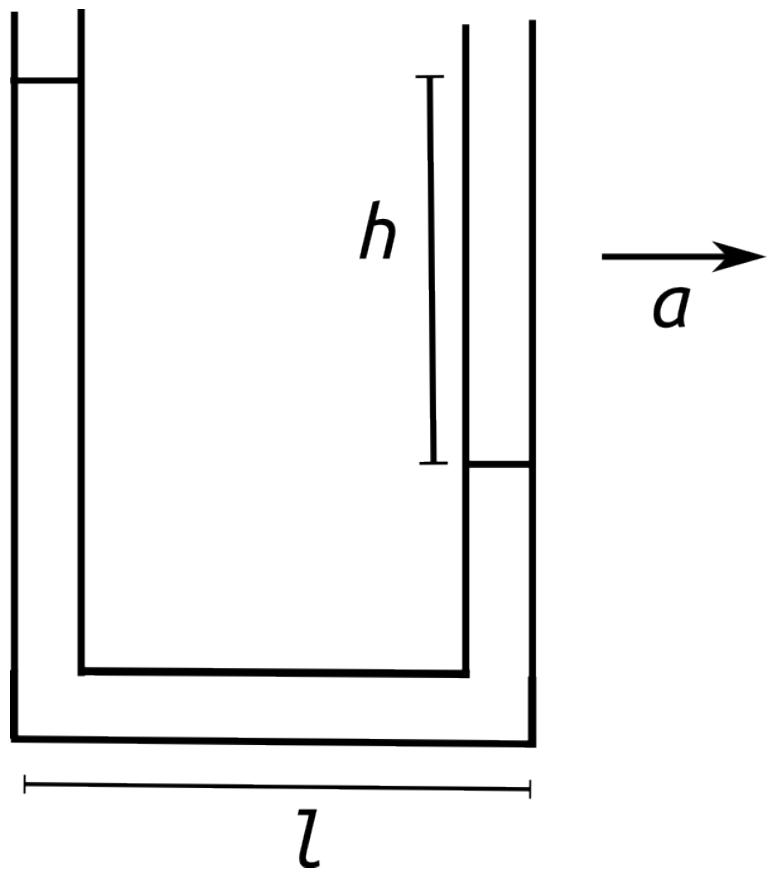
\includegraphics[width=5cm]{TuboU}
\caption{}
\label{figTuboU}
\end{center}
\end{figure}





\end{document}

